
\section{Gesture Categories}
Gestures are categorized into \textit{static gestures} and \textit{dynamic gestures}. A Group of static gestures consists of fixed gestures, where they are not relative to time. A group of dynamic gestures, on the other hand, are time-varying. These classes can be further subdivided into a set of gestures distinct by their purpose.


\begin{itemize}
	\item \textbf{Deictic gestures} involve pointing to establish the identity or spatial location of an object within the context of the application domain \cite{taxonomi}.
    \item \textbf{Manipulative gestures} mimic manipulation of a physical object, such as scaling, moving, or rotating.
    \item \textbf{Gesticulation} is commonly used along with the language group. These hand gestures are difficult to analyse.
	\item \textbf{Language group of hand gestures} form a grammatical structure for conversational style interfaces.
    \item \textbf{Semaphoric hand gestures} also may be referred to as communicative gestures, are a group of hand gestures serving as a set of symbols/commands used to interact with machines. The group consists of static hand gestures as well as dynamic hand gestures. 
\end{itemize}


\section{Tracking devices}
Hand and body gesture recognition had followed a conventional scheme of extracting key features via one or multiple preprocessing sensors and applying machine learning techniques on them \cite{avola}. The field of gesture recognition gave birth to several image processing devices yielding useful data.
We will only cover optical devices, but there are also controllers in the form of a stick with buttons, like HTC Vive, or others in the form of gloves, sending tracking information to the computer.
\subsection{Microsoft Kinect}
%=======================================================================================================================
One of them being Micorosoft Kinect, a device first released in 2010. Originally developed for gaming but eventually finding more success in academics and commercial applications, such as robotics, medicine, and health care, it led Microsoft to discontinue production of its Xbox version in 2018 and release Azure Kinect in March 2020, incorporating Microsoft Azure cloud computing functionalities.

\begin{figure}[ht]
	\centering
    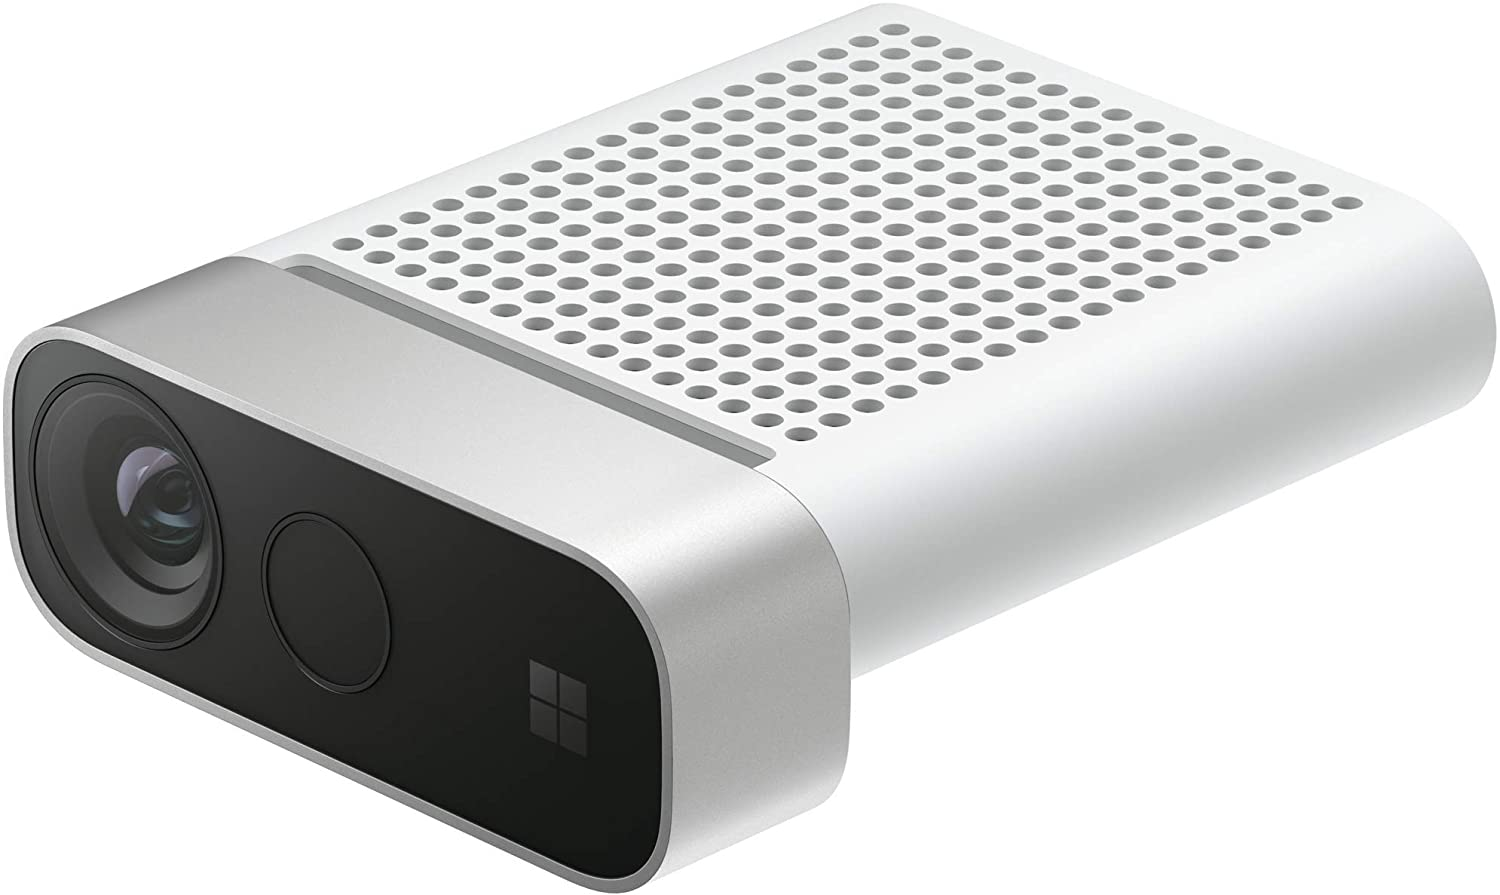
\includegraphics[width=8cm]{azure_kinect.jpg}
	\caption{Azure Kinect \cite{azurekinect_pic}}
	\label{fig:azureKincet}
\end{figure}

Azure Kinect contains a depth sensor, spatial microphone array with a video camera, and orientation sensor as a small all-in-one device with multiple modes, options, and software development kits \cite{azurekinect}.

With all that said, the primary purpose of the Kinect device overall is to interpret whole-body movement. For such, it lacks in required accuracy for hand gesture recognition, thus making it insufficient for our uses.

\subsection{Leap Motion Controller}
%=======================================================================================================================

Another option would be using a Leap Motion Controller (LMC), developed specifically to track hand movements and extract its features, such as positions of fingers, hand rotation, and others.

LMC consists of two monochromatic IR cameras and three IR LEDs (emitters). 

\begin{figure}[ht]
	\centering
    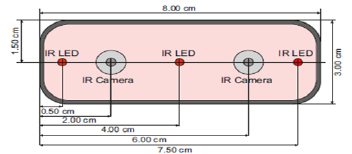
\includegraphics[width=8cm]{lmc_schematic.png}
	\caption{Schematic View of Leap Motion Controller \cite{LMCanalysis}}
	\label{fig:lmcScheme}
\end{figure}



The LMC's current API, Leap Motion Service, yields positions of extracted hand features. All the positional data about the hand and its features are represented in the coordinate system relative to the LMC's center point, positioned at top of the controller \cite{LMCanalysis}. The x- and z-axes lie in the camera sensors plane, with the x-axis running along the camera baseline. The y-axis is vertical, with positive values increasing upwards (in contrast to the downward orientation of most computer graphics coordinate systems). The z-axis has positive values increasing toward the user \cite{tomasMultileap}.

\begin{figure}[ht]
	\centering
    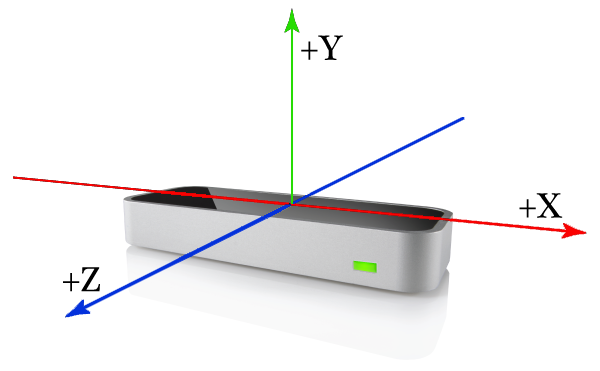
\includegraphics[width=8cm]{leap_axes.png}
	\caption{Leap Motion Controller Axes \cite{tomasMultileap}}
	\label{fig:lmcScheme}
\end{figure}

\subsection{Ultraleap Stereo IR 170}

Ultraleap Stereo IR 170, formerly known as the Leap Motion Rigel, is the successor to the Leap Motion controller.

The Stereo IR inherits Leap Motions key features but improves with a wider 170-degree field of view, more-powerful LED illuminators providing more extended tracking range, and a higher framerate when used with USB 3.0 \cite{ultraleap}, \cite{ultraleap2}.

\begin{figure}[H]
	\centering
    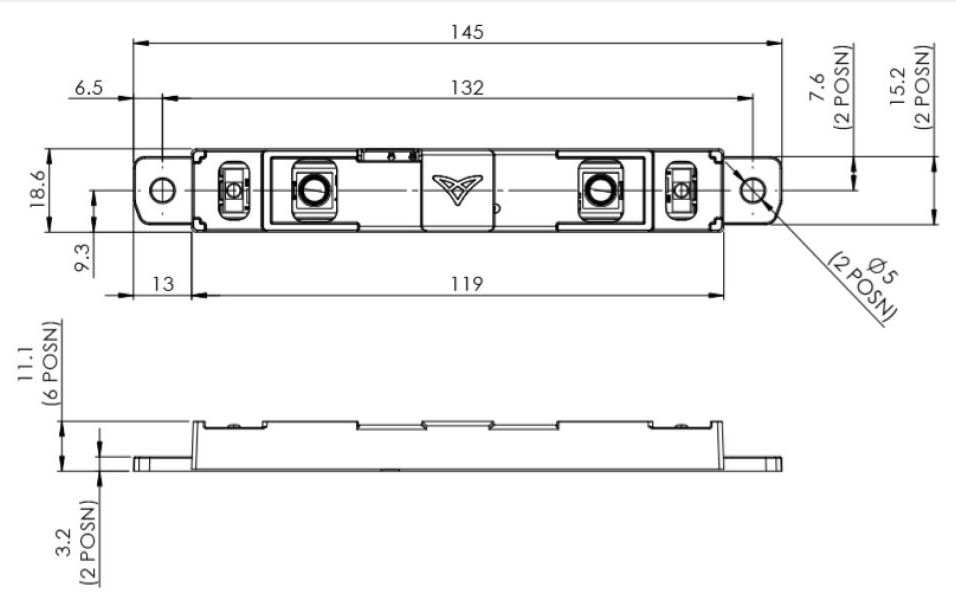
\includegraphics[width=8cm]{ultraleap_pic.jpg}
	\caption{Schematic View of Ultraleap Stereo IR 170 \cite{ultraleap}}
	\label{fig:lmcScheme}
\end{figure}

Unfortunately, Leap Motion Controller, as well as Ultraleap Stereo IR 170, has no official library for gesture recognition, limiting developers from utilizing the controller for its key features. Leap Motion provided tracking software built for virtual reality, used to have a gesture detector with its 3.0 version, but the detector is absent with the release of more accurate version 4.0.


\section{Gesture Recognition Methods
}
%=======================================================================================================================

Gestures group classification should be taken into account when choosing appropriate methods due to their time-varying properties. As previously mentioned, gestures are classified into static and dynamic groups. 

\subsection{Static Gesture Recognition}

One of the commonly used methods for static gesture recognition is \textit{Support Vector Machine} (SVM), an algorithm used for both regression and classification tasks. But overall, it is widely used in classifications. SVM's goal is to find a \textit{hyperplane} in N-dimension space, N being the number of features, that distinctively classifies data points \cite{svmIntroToML}. \textit{Hyperplanes} are decision boundaries between data points and optimal \textit{hyperplane} is the one with maximal separation, \textit{margin}, between classes \cite{savaris}.

Chen and Tseng \cite{chentseng} presented an SVM solution for multi-angle hand gesture recognition for rock paper scissors using images from a web camera. The training dataset consisted of 420 images and a testing set of 120 images. 
Datasets were collected from 5 different people for the right hand only and achieving 95\%. The classifier still managed to recognize left-hand gestures with 90\% accuracy. 

Domino et al. \cite{dominokinect} utilized SVM with Microsoft Kinect sensors. Extracting hand features, fingertips, and center of the hand, from the depth map and feeding the data into SVM. Achieving 99.5\% recognition rate on the dataset provided by Ren et Al. \cite{dominokinect_data}. The dataset consists of 10 different gestures performed by ten different people repeatedly each ten times, a total of 1000 different depth maps.

Mapari and Kharat \cite{mapari} on the other hand, proposed a method to recognize American Sign Language (ASL) with an \textit{Feed-forward network} using \textit{Multilayer Perceptron (MLP)}, extracting data from LMC and computing 48 features (18 positional values, 15 distance values, and 15 angle values) for 4672 collected signs (146 users for 32 signs). The average classification accuracy is 90\%.

\subsection{Dynamic Gesture Recognition}

Katia et al. \cite{katiacnn} proposed a method classifying dynamic gestures acquired through LMC with a CNN.
Adopting a modified version of ResNet-50 architecture, a 50 layers deep CNN, removing the last fully connected layer and adding a new layer with as many neurons as the considered collection of gesture classes. 
The acquired gesture information is converted into hand joints color images. The variation of hand joint positions during the gesture is projected on a plane, and temporal information is represented with the color intensity of the projected points. The trained model achieved 91\% classification accuracy on the LMDHG dataset \cite{lmdhg}.

Ameur et al. \cite{ameur} presented a solution using an SVM classifier used with LMC acquired data, (X, Y, Z) coordinates of fingertips and palm center. The experimental results show an accuracy of 81\% on a dataset containing 11 actions, performed by ten different subjects, having in total 550 samples.

Yang L., Chen J., and Zhu W. \cite{bidirect_dynam} used two-layer Bidirectional RNN in combination with an LMC to classify dynamic hand gestures represented by sets of feature vectors (fingertip distance, angle, height, the angle of adjacent fingertips and the coordinates of the palm). The proposed method has been tested on modified American Sign Language (ASL) datasets with 360 samples and the Handicraft‐Gesture dataset with 480 samples, both containing only dynamic gestures and achieving 90\% and 92\% accuracy. The LMC was used only for data acquisition. The architecture was not further tested in real-time environment and also the performance on static gestures is unclear since both benchmarked datasets were stripped of any static gesture. \cite{bidirect_dynam}

\subsection{Proposed LSTM solution}

Many of the proposed methods focus either on static gesture recognition or dynamic gesture recognition, but very few of them are actually utilized for both types at the same time. 

Avola D., Bernardi M. et al. proposed a method in \cite{avola} using LSTM, specifically Deep LSTM (DLSTM), and LMC to recognize sign language and semaphoric hand gestures. It uses a hand skeleton extracted by an LMC and considers angles formed by a specific subset of hand joints. The presented method reached 96\% accuracy in its predictions.

The LMC was used only to collect data for training. The method was not tested in real-time environment, it is yet to be explored whether it will.

Consider each hand gesture to be represtend as set $X = \{x_0, x1, ..., x_{T-1}\}$ of feature vectors, in predetermined interval $\Theta$ size T, T being the number of time instances, in which features are extraxted by LMC. DLSTM is applied to obtain series of output probability vectors $Y = \{y_0, y1, ..., y_{T-1}\}$. At last the gesture classification is performed by a \textit{softmax} layer using $n = |C|$, where C being the set of considered hand gestures \cite{avola}.

\begin{figure}[ht]
	\centering
    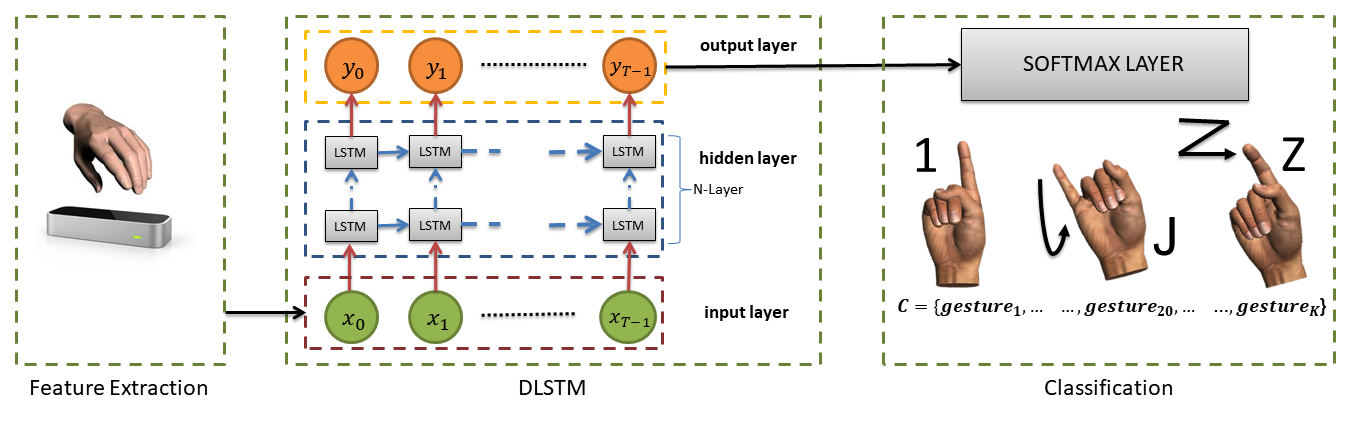
\includegraphics[width=13cm]{avola_structure.png}
	\caption{Logical structure of the proposed method \cite{avola}}
	\label{fig:lstm_gesture_structure}
\end{figure}

\subsubsection{Feature Extraction}
\label{sec:feature_extraction}

A hand gesture can be considered to be composed of different poses, where particular angles characterize each pose. Each feature vector $x_t \in X$ consists mostly of internal angles, finger segments, palm position, and fingertip positions.

\begin{figure}[ht]
	\centering
    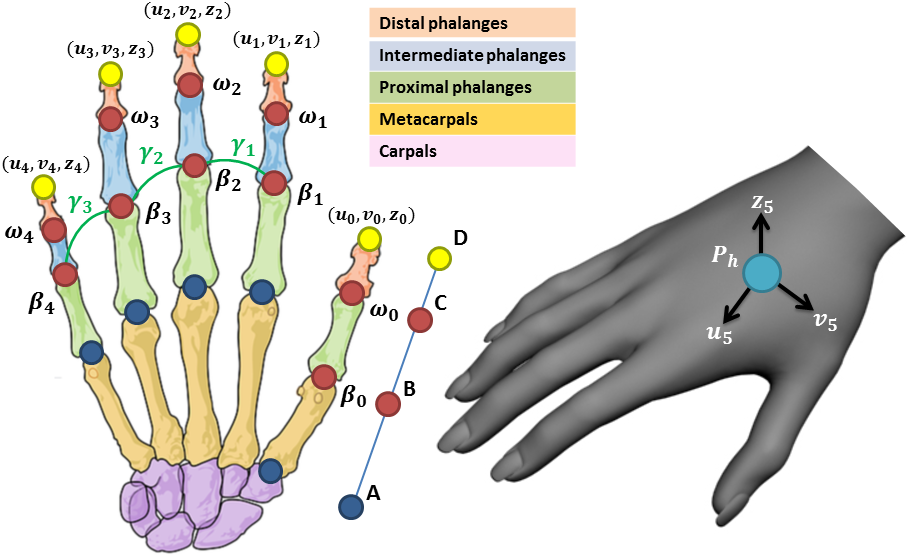
\includegraphics[width=9cm]{avola_angles.png}
	\caption{Internal angles of hand joints \cite{avola}}
	\label{fig:lstm_angles}
\end{figure}

As seen in Figure \ref{fig:lstm_angles}, each finger can be represented as set of segments:
\begin{itemize}
	\item $\overline{AB}$, proximal phalax, or metacarpal in case of thumb
	\item $\overline{BC}$, intermediate phalanx, or proximal phalanx in case of thumb
	\item $\overline{CD}$, distal phalanx
\end{itemize}

These set of segments are then used to calculate internal angles of considered finger:
\begin{itemize}
    \item internal angles $\omega_1, \omega_2, \omega_3, \omega_4$ between distal phalanges and intermediate phalanges. Internal angle $\omega_0$ of the thumb is calculated between distal phalanx and proximal phalanx.
	
	\begin{equation}
		{\omega_{j \in \{0, ..., 4\}} = \frac{\overline{BC} \cdot \overline{CD}}{|\overline{BC}| \cdot |\overline{CD}|}}
	\end{equation}

    \item internal angles $\beta_1, \beta_2, \beta_3, \beta_4$ between intermediate phalanges and proximal phalanges. Internal angle $\beta_0$ of the thumb is calculated between proximal phalanx and metacarpal.
	
	\begin{equation}
		{\beta_{j \in \{0, ..., 4\}} = \frac{\overline{AB} \cdot \overline{BC}}{|\overline{AB}| \cdot |\overline{BC}|}}
	\end{equation}
	
    \item intra-finger angles $\gamma_1, \gamma_2, \gamma_3$ are angles between two neighboring fingers, where considered fingers are: the pointer finger between middle finger, the middle finger and the ring finger, and the ring finger with a pinky finger. The infra-finger angles are used to handle special static gestures,  for example, an open palm and a pop culture "Spock" greeting.
\end{itemize}


3D displacements of palm and fingertip positions serve to help classify dynamic hand gestures, where the movement is performed in 3D space.


\begin{itemize}
	\item palm central point coordinates $P_h = (u_5, v_5, z_5)$ help to track the hand transition in the 3D space.
	\item finger tip positions $u_l, v_l, z_l$, $l \in {0, ..., 4}$ help to track the hand rotation in 3D space.
\end{itemize}

All above features form the input vector $x_t$ passed to DLSTM at time $t$.

\begin{equation}
	{x_t = \{\omega_0, ...,\omega_4, \beta_0, ..., \beta_4, u_0,v_0,z_0, ..., u_5,v_5,z_5, \gamma_1, \gamma_2, \gamma_3\}}
\end{equation}

\subsubsection{Optimal Number of Stacked LSTMs}
\label{sec:dlstm_params}

Several tests were performed to find the optimal number of stacked LSTMs. The results showed that having 4 LSTM layers proved to achieve the best accuracy by using 800 \textit{epochs}, the number of times the learning algorithm goes through the complete training dataset. Although it was possible to get the same results with 5 or 6 stacked LSTM layers, only due to using 1600 and 1800 epochs, thus increasing the training time \cite{avola}. 

\begin{figure}[ht]
	\centering
    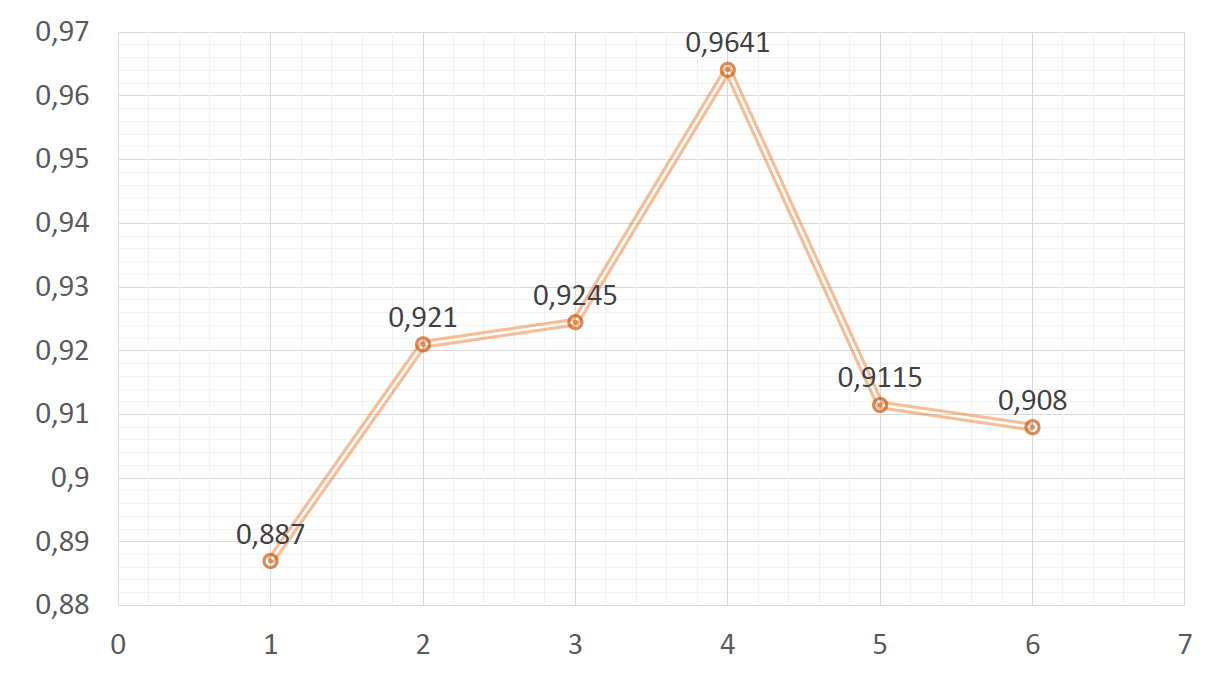
\includegraphics[width=9cm]{DLSTM_800_epochs.png}
	\caption{Model accuracy by using 800 epochs \cite{avola}}
	\label{fig:DLSTM_800_epochs}
\end{figure}

\begin{figure}[ht]
	\centering
    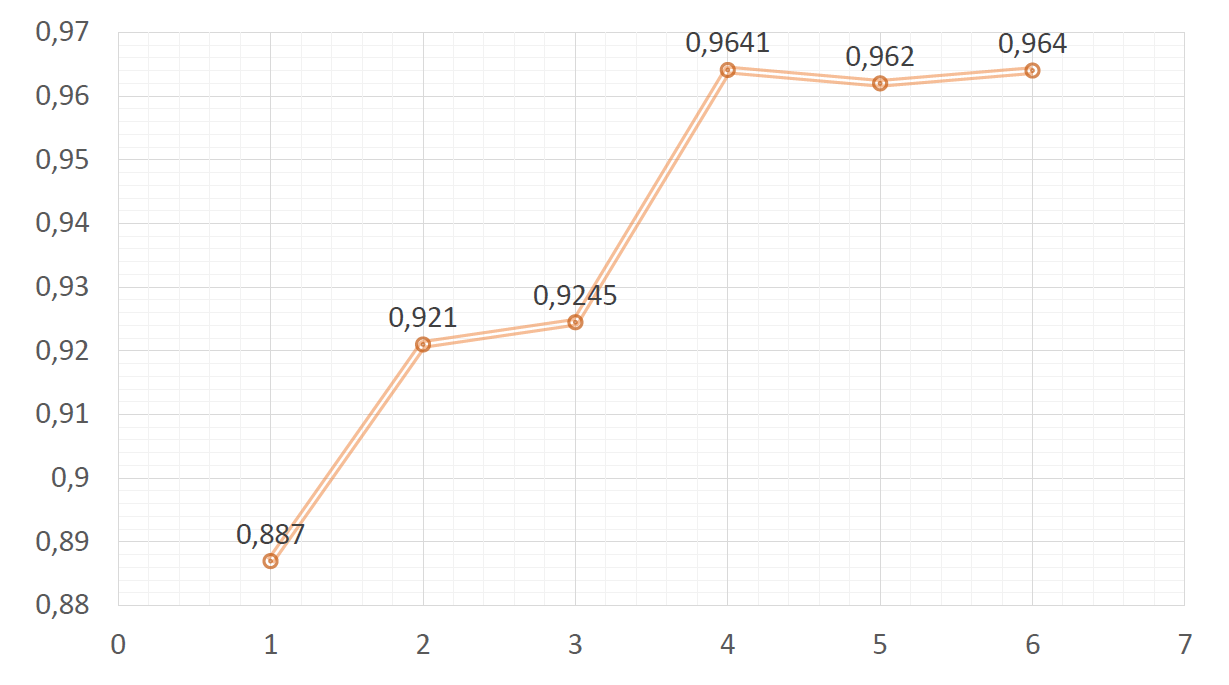
\includegraphics[width=9cm]{DLSTM_1600_epochs.png}
	\caption{Model accuracy by using 1600 epochs for 5 LSTM layers and 1800 epochs for 6 LSTM layers \cite{avola}}
	\label{fig:DLSTM_1600_epochs}
\end{figure}

The \textit{learning rate} was set to 0.0001 after large empirical tests. The learning rate determines how much the newly acquired information about the weights will influence their updating. If the learning rate is too low, it will require more time to converge towards the local minimum, while if the rate is too large, it may overstep the local minimum \cite{avola}.

\subsubsection{Sampling Process}

One gesture can be performed differently by each person, and all collected frame sequences must be composed of the same number of T samples. The proposed solution would collect data only in most significant T time instances, $t \in \Theta$ is considered significant if the joint angle and the central palm point coordinate $P_h$ differs substantially between $t$ and $t+1$.

To explain more specifically, let $f_{\omega_i}(t)$, $f_{\beta_i}(t)$, $f_{\gamma_j}(t)$ be functions representing values of $\omega_i$, $\beta_i$, $\gamma_j$ angles at time $t$, where $0 \leq i \leq 4$ and $1 \leq j \leq 3$. Coordinates of $P_h$ may be $\phi$ and coordinates at time $t$ may be represented as $f_{\phi}(t)$. Then the Savitzky-Golay filter \cite{savitzkty} is applied on each of the named functions, $f_g(t)$, $g \in G = \{\omega_i,\beta_i, \gamma_j, \phi\}$. Svaitzky-Golay is a digital filter used to smooth a set of digital data in order to increase the signal-to-noise ratio without distorting the signal itself. Local extremes of each $f_g(t)$ are to be indentified as significant time variations and all time instances $t$, associated with at least one of these local maximum and minimum of feature $g$, form a new set $\Theta^*$, representing candidates of possible important time instances to be sampled. 

\begin{figure}[h]
	\centering
    \subfloat[\centering Feature $\omega_1$]{{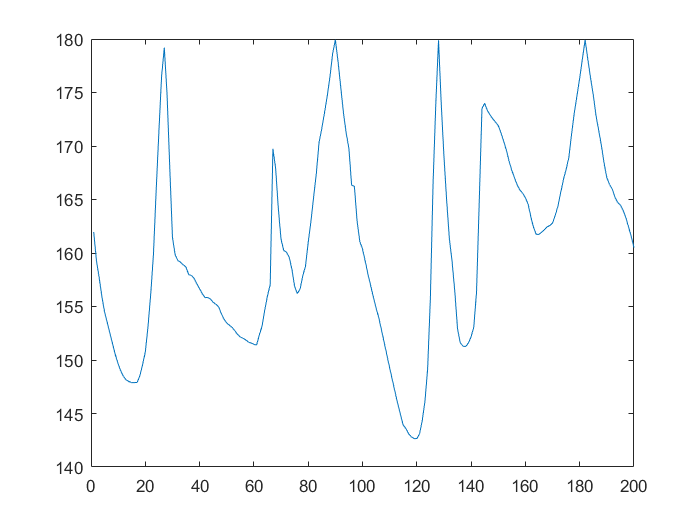
\includegraphics[width=6cm]{avola_sign.png}}}%
    \qquad
    \subfloat[\centering Feature $\omega_1$ after Savitzky-Golay filtering]{{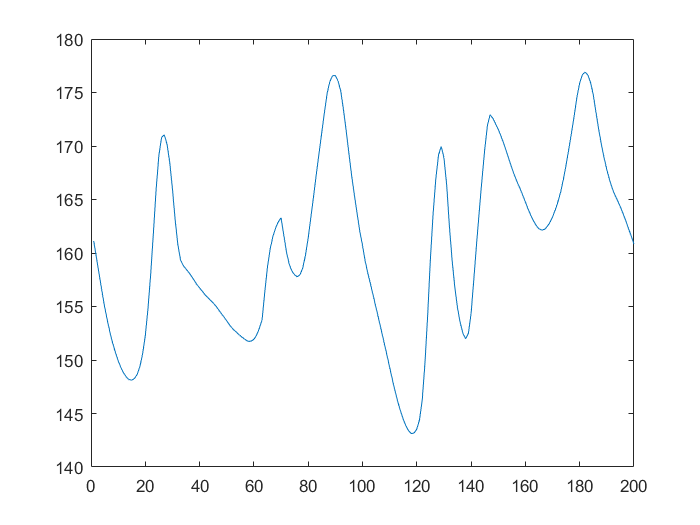
\includegraphics[width=6cm]{avola_sign_smooth.png}}}%
    \caption{Sampling example of feature $\omega_1$}
\end{figure}

Depending on the cardinality of the newly acquired set $\Theta^*$, the following cases must be considered:

\begin{itemize}
	\item $|\Theta^*| < T$, the remaining samples $(|\Theta^*|-T)$ are picked randomly from the original set $\Theta$
	\item $|\Theta^*| > T$, only some of significant time instances for each $g$ feature are picked to be sampled. Let $\Theta_g \subseteq \Theta^*$ be a set of significant time instances for feature $g$. The number of instances $T_g$ to be sampled is chosen according to the ratio $|\Theta_g|:|\Theta^*| = T_g:T$, where the sum $\sum_{g \in G}{T_g} = T$ must be preserved \cite{avola}.
\end{itemize}


